\documentclass[PhD-Yoann-Dupont.tex]{subfiles}
\begin{document}

Dans cette section, nous nous baserons essentiellement sur les travaux de \citet{cori2002constitution} afin de décrire le domaine du traitement automatique des langues (TAL).

Le TAL est un domaine de recherche ayant «\ quatre principaux pôles disciplinaires autour duquel il gravite : - la linguistique ; - l'informatique ; - les mathématiques [...] ; - l'intelligence artificielle\ » \citep{cori2002constitution}. Donner une définition précise et exacte de ce qu'est le TAL n'est pas simple, les nombreux termes proposés au fil des années témoignent de cette difficulté \citep{vauquois1969dix,cori2002constitution}. Nous emploierons ici la définition suivante :

\begin{quote}«\ Le TAL est l'ensemble des méthodes permettant de traiter de manière automatique les données exprimées dans une langue\ » (basé sur \citet{cori2002constitution,fuchs2004traitement})\end{quote}

Le TAL contient entre autres quatre grands domaines de recherches dans lesquels peuvent être classés les différentes tâches :
\begin{itemize}
    \item le traitement du signal : traite les données sous leur format le plus brut, comme le signal sonore ou des images/scans de textes écrits. Le but principal du traitement du signal est de transformer ces données sous une forme utilisable par d'autres outils informatiques ;
    \item la syntaxe : vise à fournir une analyse des données selon les règles de grammaire de la langue ;
    \item l'extraction d'information (EI) : les documents traités contiennent des éléments, traitent d'un sujet global, etc. Le but de l'EI est de récupérer ces informations intéressantes. \citet{mccallum2005information} parle de «\ distiller des données structurées de textes non-sructurés\ »;
    \item la sémantique : représente l'ensemble des traitements qui demandent une compréhension des données traitées.
\end{itemize}

Ces quatres axes principaux du TAL sont illustrés sur la figure \ref{fig:tal-timeline}, chacun de ces axes ayant des exemples de tâches en faisant parti.

\begin{figure}[ht!]
    \centering
    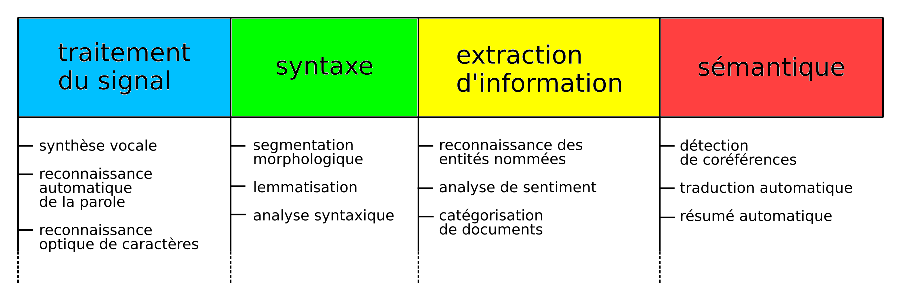
\includegraphics[scale=1.0]{images/TAL/frise1-TAL-couleurs}
    \caption{les quatre champs de recherche principaux actuels du TAL ainsi que des exemples de tâches spécifiques à chacun de ces champs.}
    \label{fig:tal-timeline}
\end{figure}

Cette thèse traite principalement la reconnaissance des entités nommées, qui s'inscrit dans le domaine de l'extraction d'information, que nous détaillons dans la section \ref{sec:EI-introduction}.

\end{document}